%run latex file, dvips file, ps2eps file

%\documentclass{article}
%\documentclass{pnastwo}
\documentclass{article}
% amsmath package, useful for mathematical formulas
%\usepackage{amsmath}
% amssymb package, useful for mathematical symbols
%\usepackage{amssymb}
\usepackage{amsmath,amssymb,mathrsfs}
% graphicx package, useful for including eps and pdf graphics
% include graphics with the command \includegraphics
\usepackage{graphicx,float,caption,color,dsfont}
\usepackage[top=2.0cm, right=2.0cm, left=2.0cm, bottom=2.0cm]{geometry}

%\usepackage{PNAStwoF}

% cite package, to clean up citations in the main text. Do not remove.
\usepackage{cite}

\usepackage{color} 

\usepackage{tikz} 
\sloppy

% \fontencoding{T1}
% \fontfamily{times}
% \fontseries{m}
% \fontshape{n}
% \fontsize{9}{11}
% \selectfont


\definecolor{monVert}{RGB}{120,212,144}
\tikzstyle{erlang} = [draw=gray!90, dashed,rectangle, minimum height=4em, minimum width=8em]
%\tikzstyle{erlang} = [draw, fill=blue!20, rectangle, minimum height=2em, minimum width=3em]
\tikzstyle{erlang_2} = [draw=gray!90,dashed,  rectangle, minimum height=4em, minimum width=12em]
%\tikzstyle{erlang_2} = [draw, fill=monVert, rectangle, minimum height=2em, minimum width=3em]
\tikzstyle{expo} = [draw, fill=orange!25,draw=orange!80, circle,minimum height=2em]
%\tikzstyle{expo} = [draw, fill=blue!20, circle,minimum height=2em]
\tikzstyle{expo_2} = [draw, fill=gray!10, circle,minimum height=2em]
\tikzstyle{output} = [coordinate]


\usetikzlibrary{arrows,snakes,backgrounds,shapes}

\begin{document}
  \thispagestyle{empty}
  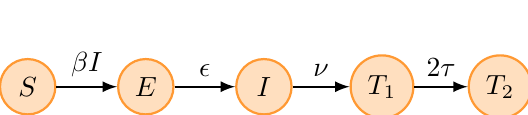
\begin{tikzpicture}[node distance=1.5cm, auto,>=latex, thick]
    % We need to set at bounding box first. Otherwise the diagram
    % will change position for each frame.
   % \path[use as bounding box] (-1,0) rectangle (10,-2);
    \path[use as bounding box] (0,0) rectangle (6,0.75);
    \node [expo] (sain) {$S$};
    \node [expo, right of=sain] (expose) {$E$};
    \node [expo, right of=expose] (infecte) {$I$};
    \node [expo, right of=infecte] (immunise1) {$T_1$};
    \node [expo, right of=immunise1] (immunise) {$T_2$};

    \node [expo, right of=immunise] (longue) {$L$};

% Once the nodes are placed, connecting them is easy. 
    \draw [->] (sain) -- node {$\beta I$} (expose);
    \draw [->] (expose) -- node{$\epsilon$}(infecte);
    \draw [->] (infecte) -- node{$\nu$}(immunise1);
    \draw [->] (immunise1) -- node{$2\tau$}(immunise);
    \draw [->] (immunise) -- node{$2\tau\alpha$}(longue);
    \draw [->] (immunise) -- +(0,-0.75) -| node[near start,below] {$(1-\alpha)\tau$}(sain);
  \end{tikzpicture}
\end{document}
